% (find-LATEX "2022-1-C2-VR.tex")
% (defun c () (interactive) (find-LATEXsh "lualatex -record 2022-1-C2-VR.tex" :end))
% (defun C () (interactive) (find-LATEXsh "lualatex 2022-1-C2-VR.tex" "Success!!!"))
% (defun D () (interactive) (find-pdf-page      "~/LATEX/2022-1-C2-VR.pdf"))
% (defun d () (interactive) (find-pdftools-page "~/LATEX/2022-1-C2-VR.pdf"))
% (defun e () (interactive) (find-LATEX "2022-1-C2-VR.tex"))
% (defun o () (interactive) (find-LATEX "2022-1-C2-P2.tex"))
% (defun u () (interactive) (find-latex-upload-links "2022-1-C2-VR"))
% (defun v () (interactive) (find-2a '(e) '(d)))
% (defun d0 () (interactive) (find-ebuffer "2022-1-C2-VR.pdf"))
% (defun cv () (interactive) (C) (ee-kill-this-buffer) (v) (g))
%          (code-eec-LATEX "2022-1-C2-VR")
% (find-pdf-page   "~/LATEX/2022-1-C2-VR.pdf")
% (find-sh0 "cp -v  ~/LATEX/2022-1-C2-VR.pdf /tmp/")
% (find-sh0 "cp -v  ~/LATEX/2022-1-C2-VR.pdf /tmp/pen/")
%     (find-xournalpp "/tmp/2022-1-C2-VR.pdf")
%   file:///home/edrx/LATEX/2022-1-C2-VR.pdf
%               file:///tmp/2022-1-C2-VR.pdf
%           file:///tmp/pen/2022-1-C2-VR.pdf
% http://angg.twu.net/LATEX/2022-1-C2-VR.pdf
% (find-LATEX "2019.mk")
% (find-sh0 "cd ~/LUA/; cp -v Pict2e1.lua Pict2e1-1.lua Piecewise1.lua ~/LATEX/")
% (find-sh0 "cd ~/LUA/; cp -v Pict2e1.lua Pict2e1-1.lua Pict3D1.lua ~/LATEX/")
% (find-sh0 "cd ~/LUA/; cp -v C2Subst1.lua C2Formulas1.lua ~/LATEX/")
% (find-CN-aula-links "2022-1-C2-VR" "2" "c2m221vr" "c2vr")

% «.defs»		(to "defs")
% «.defs-T-and-B»	(to "defs-T-and-B")
% «.title»		(to "title")
% «.escadas-defs»	(to "escadas-defs")
% «.questao-1»		(to "questao-1")
% «.questao-1-gab»	(to "questao-1-gab")
% «.questao-2»		(to "questao-2")
% «.questao-2-gab»	(to "questao-2-gab")
% «.questao-3»		(to "questao-3")
%
% «.djvuize»		(to "djvuize")



% <videos>
% Video (not yet):
% (find-ssr-links     "c2m221vr" "2022-1-C2-VR")
% (code-eevvideo      "c2m221vr" "2022-1-C2-VR")
% (code-eevlinksvideo "c2m221vr" "2022-1-C2-VR")
% (find-c2m221vrvideo "0:00")

\documentclass[oneside,12pt]{article}
\usepackage[colorlinks,citecolor=DarkRed,urlcolor=DarkRed]{hyperref} % (find-es "tex" "hyperref")
\usepackage{amsmath}
\usepackage{amsfonts}
\usepackage{amssymb}
\usepackage{pict2e}
\usepackage[x11names,svgnames]{xcolor} % (find-es "tex" "xcolor")
\usepackage{colorweb}                  % (find-es "tex" "colorweb")
%\usepackage{tikz}
%
% (find-dn6 "preamble6.lua" "preamble0")
%\usepackage{proof}   % For derivation trees ("%:" lines)
%\input diagxy        % For 2D diagrams ("%D" lines)
%\xyoption{curve}     % For the ".curve=" feature in 2D diagrams
%
\usepackage{edrx21}               % (find-LATEX "edrx21.sty")
\input edrxaccents.tex            % (find-LATEX "edrxaccents.tex")
\input edrx21chars.tex            % (find-LATEX "edrx21chars.tex")
\input edrxheadfoot.tex           % (find-LATEX "edrxheadfoot.tex")
\input edrxgac2.tex               % (find-LATEX "edrxgac2.tex")
%\usepackage{emaxima}              % (find-LATEX "emaxima.sty")
%
%\usepackage[backend=biber,
%   style=alphabetic]{biblatex}            % (find-es "tex" "biber")
%\addbibresource{catsem-slides.bib}        % (find-LATEX "catsem-slides.bib")
%
% (find-es "tex" "geometry")
\usepackage[a6paper, landscape,
            top=1.5cm, bottom=.25cm, left=1cm, right=1cm, includefoot
           ]{geometry}
%
\begin{document}

\catcode`\^^J=10
\directlua{dofile "dednat6load.lua"}  % (find-LATEX "dednat6load.lua")
%L dofile "Piecewise1.lua"           -- (find-LATEX "Piecewise1.lua")
%L dofile "QVis1.lua"                -- (find-LATEX "QVis1.lua")
%L dofile "Pict3D1.lua"              -- (find-LATEX "Pict3D1.lua")
%L dofile "C2Formulas1.lua"          -- (find-LATEX "C2Formulas1.lua")
%L Pict2e.__index.suffix = "%"
\pu
\def\pictgridstyle{\color{GrayPale}\linethickness{0.3pt}}
\def\pictaxesstyle{\linethickness{0.5pt}}
\def\pictnaxesstyle{\color{GrayPale}\linethickness{0.5pt}}
\celllower=2.5pt

% «defs»  (to ".defs")
% (find-LATEX "edrx21defs.tex" "colors")
% (find-LATEX "edrx21.sty")

\def\u#1{\par{\footnotesize \url{#1}}}

\def\drafturl{http://angg.twu.net/LATEX/2022-1-C2.pdf}
\def\drafturl{http://angg.twu.net/2022.1-C2.html}
\def\draftfooter{\tiny \href{\drafturl}{\jobname{}} \ColorBrown{\shorttoday{} \hours}}

% «defs-T-and-B»  (to ".defs-T-and-B")
% (c3m202p1p 6 "questao-2")
% (c3m202p1a   "questao-2")
\long\def\ColorOrange#1{{\color{orange!90!black}#1}}
\def\T(Total: #1 pts){{\bf(Total: #1)}}
\def\T(Total: #1 pts){{\bf(Total: #1 pts)}}
\def\T(Total: #1 pts){\ColorRed{\bf(Total: #1 pts)}}
\def\B       (#1 pts){\ColorOrange{\bf(#1 pts)}}



%  _____ _ _   _                               
% |_   _(_) |_| | ___   _ __   __ _  __ _  ___ 
%   | | | | __| |/ _ \ | '_ \ / _` |/ _` |/ _ \
%   | | | | |_| |  __/ | |_) | (_| | (_| |  __/
%   |_| |_|\__|_|\___| | .__/ \__,_|\__, |\___|
%                      |_|          |___/      
%
% «title»  (to ".title")
% (c2m221vrp 1 "title")
% (c2m221vra   "title")

\thispagestyle{empty}

\begin{center}

\vspace*{1.2cm}

{\bf \Large Cálculo 2 - 2022.1}

\bsk

Prova de reposição (VR)

\bsk

Eduardo Ochs - RCN/PURO/UFF

\url{http://angg.twu.net/2022.1-C2.html}

\end{center}

\newpage


% «escadas-defs»  (to ".escadas-defs")
% (c2m221p1p 7 "escadas-defs")
% (c2m221p1a   "escadas-defs")

%L PictList{}:setbounds(v(0,-4),v(13,4)):pgat("pgatc"):sa("respgrid"):output()
%L
%L hx = function (x, y) return format(" (%s,%s)c--(%s,%s)o", x-1,y, x,y) end
%L hxs = function (ys)
%L     local str = ""
%L     for x,y in ipairs(ys) do str = str .. hx(x, y) end
%L     return str
%L   end
%L mtintegralspec2 = function (x0, y0, Dys, dot0, dot1)
%L     local mkxy = function (x,y) return format("(%d,%d)", x, y) end
%L     local xys = { mkxy(x0,y0) .. (dot0 or "") }
%L     local x,y = x0,y0
%L     for i,Dy in ipairs(Dys) do
%L       x = x + 1
%L       y = y + Dy
%L       table.insert(xys, mkxy(x,y))
%L     end
%L     xys[#xys] = xys[#xys] .. (dot1 or "")
%L     return table.concat(xys, "--")
%L   end
%L
%L ysf   = {2, 1, 0, -1, -2,   0, 1, 2, 1, 0,  -2, -1, 0, 1, 2}
%L ysf   = {2, 1, 0, -1, -2,   2, 0, 2,  -2, -1, 0, 1, 2}
%L ysf_  = {1, 2, 1, 0, -1, -2, -1}
%L ysg   = {0, 1, 2, 3, -2, -1,  0, -1, -2, 3, 2, 1, 0}
%L ysg_  =                         {-1, -2, 3, 2, 1}
%L 
%L specf = hxs(ysf)
%L specF = mtintegralspec2(0, -2, ysf, "", "")
%L specH = mtintegralspec2(0, -4, ysf_, "", "o\n") ..
%L         mtintegralspec2(7,  1, ysg_, "o", "")
%L specM = mtintegralspec2(0, -4, ysf_, "", "o\n") ..
%L         mtintegralspec2(7,  2, ysg_, "o", "")
%L -- = specH
%L -- = specM
%L pwsf  = PwSpec.from(specf)
%L pwsF  = PwSpec.from(specF)
%L pwsH  = PwSpec.from(specH)
%L pwsM  = PwSpec.from(specM)
%L pf    = pwsf:topict():setbounds(v(0,-2),  v(13,2)):pgat("pgatc")
%L pF    = pwsF:topict():setbounds(v(0,-2),  v(13,2)):pgat("pgatc")
%L pH    = pwsH:topict():setbounds(v(0,-4),  v(12,4)):pgat("pgatc")
%L pM    = pwsM:topict():setbounds(v(0,-4),  v(12,5)):pgat("pgatc")
%L pf:sa("Fig f"):output()
%L pF:sa("Fig F"):output()
%L pH:sa("Fig H"):output()
%L pM:sa("Fig M"):output()
%L
%L PictList{}:setbounds(v(0,-4),v(13,4)):pgat("pgatc"):sa("respgrid"):output()

\pu

\unitlength=10pt

% «questao-1»  (to ".questao-1")
% (c2m221vrp 2 "questao-1")
% (c2m221vra   "questao-1")

{\bf Questão 1}


\scalebox{0.8}{\def\colwidth{8cm}\firstcol{

\hbox{\T(Total: 1.0 pts)}

\msk

Sejam:

$f(x) \;=\; \ga{Fig f}$

e $F(x) = \D \Intt{6}{x}{f(x)}$.

\msk

Faça o gráfico da $F(x)$.


}\anothercol{

\unitlength=8pt

\vspace*{-0cm}

$\ga{respgrid}$

\bsk

$\ga{respgrid}$

\bsk

$\ga{respgrid}$

}}

\newpage

% «questao-1-gab»  (to ".questao-1-gab")
% (c2m221vrp 2 "questao-1-gab")
% (c2m221vra   "questao-1-gab")

{\bf Questão 1: gabarito}

\newpage

% «questao-2»  (to ".questao-2")
% (c2m221vrp 4 "questao-2")
% (c2m221vra   "questao-2")
% (c2m221p2p 3 "edo-2a-ordem")
% (c2m221p2a   "edo-2a-ordem")
% (c2m212introp 12 "EDOs-chutar-testar")
% (c2m212introa    "EDOs-chutar-testar")

{\bf Questão 2}

\scalebox{0.55}{\def\colwidth{10cm}\firstcol{

\hbox{\T(Total: 6.0 pts)}

Obs: esta questão é uma versão

modificada de uma questão da P2.

\msk

EDOs {\sl parecidas} com essa aqui
%
$$f''(x) + 7f'(x) + 10f(x) = 0 \qquad (*)$$

vão ser incrivelmente importantes nos cursos de Física. Algumas delas
descrevem ``oscilações amortecidas'', como esta figura:

\vspace*{-0.25cm}

% (find-pdf-page "~/LATEX/2022-1-C2/osc-amort.pdf")
$$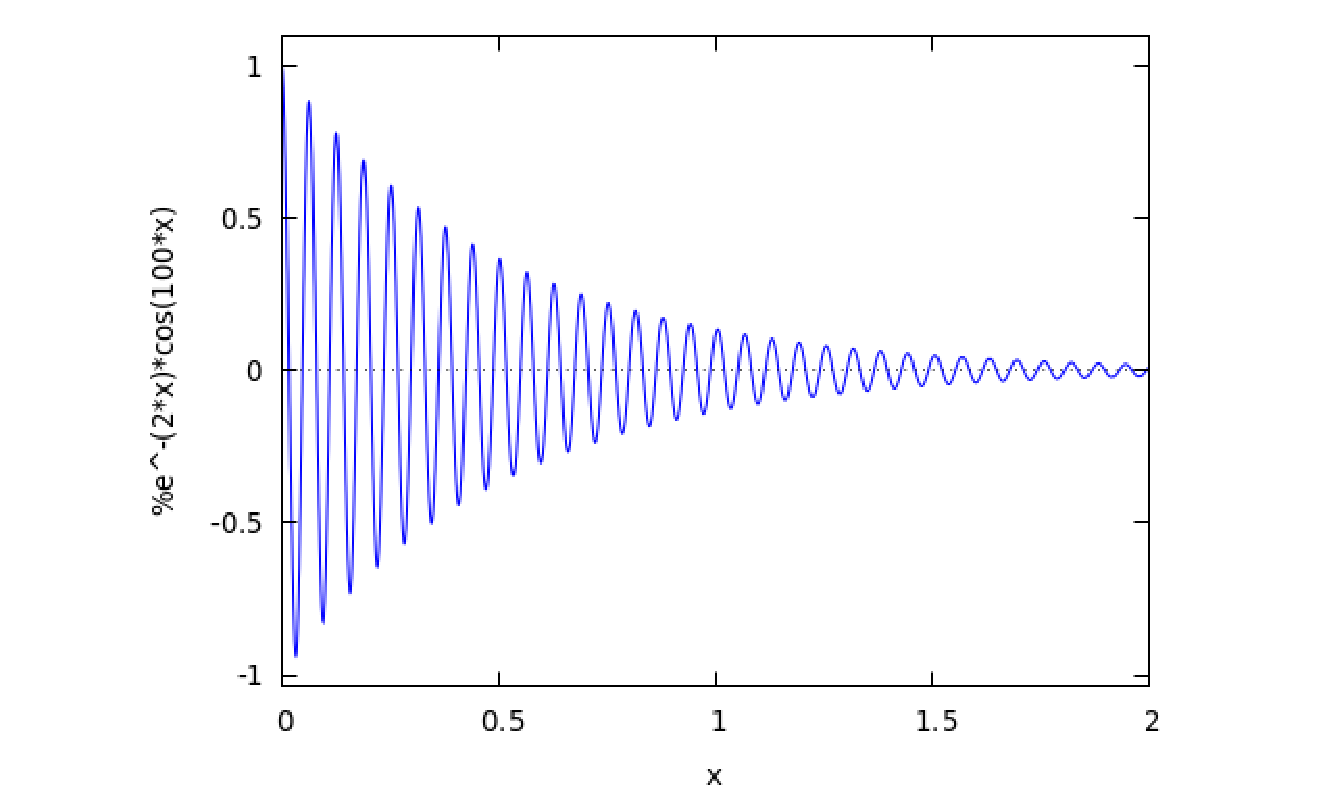
\includegraphics[width=4cm]{2022-1-C2/osc-amort.pdf}$$

\vspace*{-0.25cm}

A maioria dos livros ``normais'' de EDOs ensinam um modo de resolver a
$(*)$ que eu acho muito árido. Nesta questão você vai ver um método
pra resolver EDOs desse tipo que eu acho bem mais legal, e que eu
aprendi num curso de Álgebra Linear. Nesse método a gente trata
funções como vetores (de dimentão infinita) e a derivada como uma
transformação linear (uma ``matriz de dimensão infinita''). Quando eu
precisar enfatizar que estou ``em Álgebra Linear'' eu vou escrever $f$
e $D$ ao invés de $f(x)$ e $\ddx$.

}\anothercol{

  Isto aqui é uma demonstração quase completa do modo rápido de
  encontrar as ``soluções básicas'' e a ``solução geral'' da EDO
  $(*)$... ela é ``quase completa'' no sentido de que ela é o que as
  pessoas escrevem no quadro quando explicam esse método, mas sem a
  parte falada.
  %
  $$\scalebox{0.9}{$
    \begin{array}{rcl}
      f''(x)+7f'(x)+10f(x) &=& 0 \\
      \ddx \ddx f(x) + 7 \ddx f(x)+10f(x) &=& 0 \\
      (\ddx \ddx + 7 \ddx + 10) f(x) &=& 0 \\
      (D^2 + 7D + 10)f &=& 0 \\
      (D^2 + (2+5)D + (2·5))f &=& 0 \\
      (D+2)(D+5)f &=& 0 \\
      (D+2)(D+5)e^{-5x} &=& (D+2)(De^{-5x}+5e^{-5x}) \\
                           &=& (D+2)(-5e^{-5x}+5e^{-5x}) \\
                           &=& (D+2)0 \\
                           &=& 0 \\
      (D+5)(D+2)f &=& 0 \\
      (D+5)(D+2)e^{-2x} &=& (D+5)(De^{-2x}+2e^{-2x}) \\
                           &=& (D+5)(-2e^{-2x}+2e^{-2x}) \\
                           &=& (D+5)0 \\
                           &=& 0 \\
      (D^2 + 7D + 10)(γe^{-2x} + δe^{-5x}) &=& 0 \\
    \end{array}
    $}
    $$

    (Continua...)
}}



\newpage

% (c2m221p2p 6 "edo-2a-ordem-cont")
% (c2m221p2a   "edo-2a-ordem-cont")

{\bf Questão 2 (cont.)}

% (c2m221p2p 3 "edo-2a-ordem")
% (c2m221p2a   "edo-2a-ordem")
% (c2m212introp 12 "EDOs-chutar-testar")
% (c2m212introa    "EDOs-chutar-testar")


\scalebox{0.55}{\def\colwidth{10cm}\firstcol{

    ...e isto aqui é uma versão mais curta da demonstração da página
    anterior:

    $$\scalebox{0.8}{$
      \begin{array}{rcl}
        f''(x)+7f'(x)+10f(x) &=& 0 \\
        (D^2 + 7D + 10)f &=& 0 \\
        (D^2 + (2+5)D + (2·5))f &=& 0 \\
        (D^2 + 7D + 10)(γe^{-2x} + δe^{-5x}) &=& 0 \\
      \end{array}
      $}
    $$

    Aqui que você já tem uma certa prática com problemas de ``encontre
    a substituição certa'' você vai fazer um problema de ``encontre a
    generalização certa''. Vou explicar ele em português.

    \msk

    a) \B (0.2 pts) Você vai definir [EDOLP] -- de ``EDO linear, caso
    particular'' -- como sendo o bloco de quatro igualdades acima.
    Faça isso na notação certa, que é algo como ``[EDOLP] = ?''.

    \msk

    b) \B (2.3 pts) Depois disso você vai procurar a ``generalização
    certa'' da [EDOLP], e na ``substituição certa'' que transforma ela
    na [EDOLP]. O seu objetivo é chegar em algo da forma [EDOLG][S] =
    [EDOLP]; o nome ``[EDOLG]'' vem de ``EDO linear, caso geral''. É
    difícil chegar na [EDOLG] direto, então vou dar instruções pra
    você chegar lá por chutar-e-testar.


}\anothercol{

  Chame as suas tentativas de [EDOLG1], [EDOLG2], etc, e as suas
  substituições de [S1], [S2], etc. O seu objetivo é chegar numa
  [EDOLG${}_n$] que não tenha mais os números 2, 5, 7 e 10; eles devem
  ter sido substuídos ou por variáveis ou por expressões que dependem
  dessas variáveis.

  \msk

  O seu objetivo {\sl final} neste item é chegar num caso em que [S]
  seja só isto aqui:
  %
  $$\text{[S]} = \bmat{α:=2 \\ β:=5}$$

  E isto valha:
  %
  $$\text{[EDOLG]} \bmat{α:=2 \\ β:=5} \text{``=''} \text{[EDOLP]}$$

  Eu pus o \text{``=''} entre aspas porque você vai não chegar a algo
  exatamente igual à [EDOLP], só em algo equivalente à EDOLP... como o
  que a gente fez nos exercícios de ``justifique esse passo''.

  \msk

  % Quem for fazer a VS vai ver como nos últimos semestres a gente usou
  % essa técnica pra aprender a demonstrar algumas fórmulas das tabelas
  % de integração dos livros -- a gente começava com um caso particular
  % e ``generalizava ele do jeito certo'' depois.

}}

\newpage

{\bf Questão 2 (cont.)}

\scalebox{0.6}{\def\colwidth{9cm}\firstcol{

  c) \B (1.0 pts) Seja:
  %
  $$[S2] = \bmat{α:=3 \\ β:=4 \\ γ:=1 \\ δ:=0}$$

  Calcule o
  resultado disto aqui:
  %
  $$[\text{EDOO}] = \text{[EDOLG][S2]} = \Rq$$

  \msk

  d) \B (2.5 pts) No item (c) você definiu o [EDOO] (``outra EDO'')
  como uma sequência de quatro igualdades. Se você tiver feito tudo
  certo até aqui, e você interpretar as quatro igualdades da [EDOO] do
  jeito correto, você vai ver que elas dizem algo como:
  %
  $$\begin{tabular}{l}
      A função $f(x) = e^{20x}$ \\
      é solução da EDO \\
      $f''(x) + 42f'(x) + 99f(x) = 0$ \\
    \end{tabular}
  $$

}\anothercol{

  ...só que eu pus números errados de propósito. Descubra os números
  certos -- a única dica que eu posso dar aqui é que o 20 do $e^{20x}$
  tem que virar ou 3, ou 4, ou -3, ou -4 -- e verifique que essa
  $f(x)$ realmente é solução dessa EDO.

}}

\newpage

% «questao-2-gab»  (to ".questao-2-gab")
% (c2m221vrp 7 "questao-2-gab")
% (c2m221vra    "questao-2-gab")

{\bf Questão 2: gabarito}

\newpage

% «questao-3»  (to ".questao-3")
% (c2m221vrp 8 "questao-3")
% (c2m221vra   "questao-3")


{\bf Questão 3}


\scalebox{0.6}{\def\colwidth{9cm}\firstcol{

\hbox{\T(Total: 3.0 pts)}

\msk

Calcule as seguintes integrais indefinidas e teste os seus resultados.

a) \B (1.0 pts)
%
$$\intx{2x + \frac{4}{x^3} + \cos 4x}$$

b) \B (2.0 pts)
%
$$\intx{(3x+4)^{20}}$$

Dica pro item (b): se você souber o método de mudança de variável que
os livros usam você consegue calcular ela bem rápido usando a mudança
de variável $u=3x+4$. Dá pra calcular essa integral por
chutar-e-testar, mas dá um pouquinho mais de trabalho.


}\anothercol{

{\bf Gabarito}

(sem os testes)

\msk

a)
%
$$x^2 - \frac{2}{x^2} + \frac14 \sen 4x
$$

\bsk

b)
%
$$\frac{(3x+4)^{21}}{63}
$$


}}



% (setq eepitch-preprocess-regexp "^")
% (setq eepitch-preprocess-regexp "^%T ")
%
%T  (eepitch-maxima)
%T  (eepitch-kill)
%T  (eepitch-maxima)
%T f : 2*x + 4/(x^3) + cos(4*x);
%T integrate(f,x);
%T f : (3*x+4)^20;
%T integrate(f,x);







%\printbibliography

\GenericWarning{Success:}{Success!!!}  % Used by `M-x cv'

\end{document}

%  ____  _             _         
% |  _ \(_)_   ___   _(_)_______ 
% | | | | \ \ / / | | | |_  / _ \
% | |_| | |\ V /| |_| | |/ /  __/
% |____// | \_/  \__,_|_/___\___|
%     |__/                       
%
% «djvuize»  (to ".djvuize")
% (find-LATEXgrep "grep --color -nH --null -e djvuize 2020-1*.tex")

 (eepitch-shell)
 (eepitch-kill)
 (eepitch-shell)
# (find-fline "~/2022.1-C2/")
# (find-fline "~/LATEX/2022-1-C2/")
# (find-fline "~/bin/djvuize")

cd /tmp/
for i in *.jpg; do echo f $(basename $i .jpg); done

f () { rm -v $1.pdf;  textcleaner -f 50 -o  5 $1.jpg $1.png; djvuize $1.pdf; xpdf $1.pdf }
f () { rm -v $1.pdf;  textcleaner -f 50 -o 10 $1.jpg $1.png; djvuize $1.pdf; xpdf $1.pdf }
f () { rm -v $1.pdf;  textcleaner -f 50 -o 20 $1.jpg $1.png; djvuize $1.pdf; xpdf $1.pdf }

f () { rm -fv $1.png $1.pdf; djvuize $1.pdf }
f () { rm -fv $1.png $1.pdf; djvuize WHITEBOARDOPTS="-m 1.0 -f 15" $1.pdf; xpdf $1.pdf }
f () { rm -fv $1.png $1.pdf; djvuize WHITEBOARDOPTS="-m 1.0 -f 30" $1.pdf; xpdf $1.pdf }
f () { rm -fv $1.png $1.pdf; djvuize WHITEBOARDOPTS="-m 1.0 -f 45" $1.pdf; xpdf $1.pdf }
f () { rm -fv $1.png $1.pdf; djvuize WHITEBOARDOPTS="-m 0.5" $1.pdf; xpdf $1.pdf }
f () { rm -fv $1.png $1.pdf; djvuize WHITEBOARDOPTS="-m 0.25" $1.pdf; xpdf $1.pdf }
f () { cp -fv $1.png $1.pdf       ~/2022.1-C2/
       cp -fv        $1.pdf ~/LATEX/2022-1-C2/
       cat <<%%%
% (find-latexscan-links "C2" "$1")
%%%
}

f 20201213_area_em_funcao_de_theta
f 20201213_area_em_funcao_de_x
f 20201213_area_fatias_pizza



%  __  __       _        
% |  \/  | __ _| | _____ 
% | |\/| |/ _` | |/ / _ \
% | |  | | (_| |   <  __/
% |_|  |_|\__,_|_|\_\___|
%                        
% <make>

 (eepitch-shell)
 (eepitch-kill)
 (eepitch-shell)
# (find-LATEXfile "2019planar-has-1.mk")
make -f 2019.mk STEM=2022-1-C2-VR veryclean
make -f 2019.mk STEM=2022-1-C2-VR pdf

% Local Variables:
% coding: utf-8-unix
% ee-tla: "c2vr"
% ee-tla: "c2m221vr"
% End:
